\documentclass[12pt]{article}

\usepackage{amsfonts}
\usepackage{amsmath}
\usepackage{geometry}
\usepackage{amsthm}
\usepackage{mathrsfs}
\usepackage{xcolor,graphicx}
\usepackage{subcaption}
\usepackage{setspace}
\usepackage{amssymb}
\usepackage{footmisc}

\newgeometry{margin=1in}
\setlength\parindent{0pt}

\DeclareMathOperator{\sgn}{sgn}
\DeclareMathOperator{\Heavi}{H}
\DeclareMathOperator{\grad}{\overset{\rightharpoonup}\nabla}

\DeclareMathOperator{\Hsign}{\mathscr{H}}
\newcommand\Hank[2][]{{\left( \Hsign_{#1} #2 \right) }}

\newtheorem{theorem}{Theorem}[section]
\newtheorem{definition}[theorem]{Definition}
\newtheorem{corollary}[theorem]{Corollary}

\renewcommand{\thefootnote}{\fnsymbol{footnote}}

\begin{document}

\doublespacing
\linespread{2}

\section{Analytic Solution}

Typically, in fluid dynamics, the scalar function known as the velocity potential denoted by $\varphi$, is what is desired. Once the velocity potential is known, the system is solved because  $\grad \varphi = \bf{u}$, and in the case of a free surface, the deformation of the surface can readily be found from the velocity potential as well. The velocity potential will be found in the coming sub-chapters, and then the energy deposited into the neutron star will be calculated.

\subsection{Eigenfunctions of the Laplacian}

The first step in analytically solving for the velocity potential will be to find the eigenfunctions of Laplace's equation, $\nabla^2 \varphi = 0$, since the velocity potential is conservative. Since this is a partial differential equation we will assume the solution is the product of univariate functions, $\varphi = f(r) g(\theta) h(z) T(t)$. Expanding the Laplacian for cylindrical systems gives 
\begin{align*}
\frac{1}{r}\frac{\partial}{\partial r} \left( r \frac{\partial \varphi}{\partial r} \right) + \frac{1}{r^2} \left( \frac{\partial^2 \varphi}{\partial \theta^2} \right) + \frac{\partial^2 \varphi}{\partial z^2} = 0.
\end{align*}

The temporal component can be divided out since the Laplacian does not involve time, and will be found later on. Substituting in our assumed form, and dividing by $\varphi$, yields
\begin{align}
\label{eq:laplaciansub}
\frac{1}{fr}\frac{\partial}{\partial r}(rf') + \frac{1}{r^2}\frac{g''}{g} + \frac{h''}{h} = 0.
\end{align}

Where primes denote the derivative with respect to the function's only variable. Notice that the function $h(z)$ has been separated from both $f(r)$, and $g(\theta)$, and since each function is univariate, it must be the case that the last term is constant,
\begin{align*}
\frac{h''}{h} = k^2.
\end{align*}

We cleverly force this constant to be positive to satisfy the boundary conditions, namely, that $h(-\infty) = 0$. The most general solution to this is of course exponentials,
\begin{align*}
h(z) = Ae^{kz} + Be^{-kz}.
\end{align*}

Since the velocity potential has to vanish at negative infinity, this is simplified to
\begin{align}
\label{eq:h}
h(z) = e^{kz},
\end{align}

without loss of generality we can assume the constant is one, since it can be absorbed into $T(t)$. By substituting in $k^2$ and multiplying through by $r^2$, \eqref{eq:laplaciansub} becomes
\begin{align}
\label{eq:laplacenoh}
\frac{r}{f}\frac{\partial}{\partial r} \left( rf' \right) + k^2r^2 + \frac{g''}{g} = 0,
\end{align}

and once again, $g(\theta)$ has been separated from $f(r)$, and so the last term must be constant --
\begin{align*}
\frac{g''}{g} = -\mu^2.
\end{align*}

The constant is forced to be negative since $g(\theta)$ is expected to be periodic, and not exponential. Of course, the general solution to this differential equation is 
\begin{align*}
g(\theta) = A \sin(\mu \theta) + B \cos(\mu \theta).
\end{align*}

However, our system is cylindrically symmetric; there is no way to differentiate one value of $\theta$ to another, thus, it is expected that $\varphi$ has no $\theta$ dependence, and consequentially, $g(\theta)$ must be constant, the only way this is satisfied is if $\mu = 0$, so that
\begin{align}
\label{eq:g}
g(\theta) = 1.
\end{align}

By substituting $\mu = 0$ into \eqref{eq:laplacenoh}, and multiplying through by $f$ we obtain
\begin{align*}
r \frac{\partial}{\partial r}(rf') + (k^2r^2 - 0^2)f = 0,
\end{align*}

which indeed is Bessel's differential equation of order $0$. Therefore,
\begin{align*}
f(r) = A J_0(kr) + B Y_0(kr),
\end{align*}

but, once again, $B$ must equal zero since $Y_0(0)$ is not finite which is unphysical. The radial part thus simplifies to
\begin{align}
\label{eq:f}
f(r) = J_0(kr).
\end{align}

By combining \eqref{eq:h}, \eqref{eq:g}, and \eqref{eq:f} we find that the velocity potential is 
\begin{align*}
\varphi \propto e^{kz}T(t)J_0(kr),
\end{align*}

where $k$ is the eigenvalues. Clearly though, the only restriction on $k$ is that it must be a non-negative real number, all of which are a valid solution to Laplace's equation. Therefore, the total solution must be the sum of all of these, or since $k$ is valid within an interval, we have the integral form 
\begin{align}
\label{eq:phieigen}
\varphi = \int_0^\infty e^{kz}T(t)J_0(kr)dk.
\end{align}

The temporal component can be solved for using equations of fluid dynamics.

\subsection{Temporal Component of the Velocity Potential}

The time component of the velocity potential comes from the specific problem. In our case by linearizing, and assuming the waves have a small amplitude, we have
\begin{align*}
\left( \frac{\partial \varphi}{\partial t} + (g \eta + \Phi) \right) \bigg|_{z=0} = 0,
\end{align*}

where $\eta$ denotes the deformation of the surface. This comes from the pressure condition at the surface, and in our case, has the addition of the gravitational potential. ***Fluids book eqn 3.21 3.22*** By taking the time derivative and using the relation that
\begin{align}
\label{eq:smallamp}
\frac{\partial \eta}{\partial t} = \frac{\partial \varphi}{\partial z}
\end{align}

on the surface ***, we obtain
\begin{align}
\label{eq:presscond}
\left( \frac{\partial^2 \varphi}{\partial t^2} + g \frac{\partial \varphi}{\partial z} + \frac{\partial \Phi}{\partial t} \right) \bigg|_{z=0} = 0.
\end{align}

In order to solve this partial differential equation, we must write the gravitational potential as an infinite sum of Bessel functions to match the form of $\varphi$. We can do so using the Hankel transform using the fact that it is self-reciprocal,
\begin{align*}
\frac{\partial \Phi}{\partial t}\bigg|_{z=0} &=  \int_0^\infty \Hank{\frac{\partial \Phi}{\partial t}\bigg|_{z=0}}(k) J_0(kr) k \, dk, \\
&= G m v^2 t \int_0^\infty \Hank{\frac{1}{(r^2 + v^2 t^2)^{3/2}}}(k) J_0(kr) k \, dk. \footnote[4]{}
\end{align*}

Applying the Hankel transform *** gives
\begin{align*}
\frac{\partial \Phi}{\partial t}\bigg|_{z=0} &= G m v^2 t \int_0^\infty \frac{1}{|vt|} e^{-k|vt|} J_0(kr) k \, dk, \\
&= G m v \sgn(t) \int_0^\infty e^{-kv|t|} J_0(kr) k \, dk, 
\end{align*}

\footnotetext[4]{Note that $\int_0^\infty \sqrt{r}(r^2 + v^2 t^2)^{-3/2} dr = \Gamma^2(3/4) (\pi v^3 t^3)^{-1/2} < \infty$ for $t \neq 0$ which is not concerning since this is true almost everywhere, and so the condition in Theorem *** is satisfied.}
which we can now substitute into \eqref{eq:presscond} to obtain,
\begin{align*}
\int_0^\infty J_0(kr)  \ddot{T}(t) dk + g \int_0^\infty k J_0(kr) T(t) dk + Gmv \int_0^\infty \sgn(t) e^{-kv|t|} J_0(kr)k \, dk &= 0, \\
\text{or, } \int_0^\infty \left[ \frac{\ddot{T}(t)}{k} + gT(t) + Gmv \sgn(t) e^{-kv|t|} \right] J_0(kr) k \, dk &= 0.
\end{align*}
But, this is nothing more than the Hankel transform of the differential equation for $T$. By taking the Hankel transform of both sides we can remove the integral, giving an ordinary differential equation for the time component:
\begin{align*}
\frac{\ddot{T}(t)}{k} + gT(t) + Gmv \sgn(t) e^{-kv|t|} = 0.
\end{align*}
Clearly, the homogeneous solution is $T(t) = A \cos(\omega_k t) + B \sin(\omega_k t)$ with $\omega_k^2 = gk$. The form of this differential equations suggests the particular solution should take the form $T(t) = C e^{-kv|t|}$. Substituting this in yields
\begin{align*}
C \left(k^2 v^2 \sgn^2(t) e^{-kv |t|} + gk e^{-kv |t|} \right) &+ Gmvk \sgn(t) e^{-kv|t|} = 0.
\end{align*}
Now, by rearranging we find
\begin{align*}
C &= \frac{-Gmvk \sgn(t)}{k^2v^2 + gk}, \\
&= \frac{Gmv}{g} \frac{-\sgn(t)}{1+kv^2/g}
\end{align*}
as the coefficient, and,
\begin{align*}
T(t) = \frac{Gmv}{g} \frac{1}{1+kv^2/g} \left( -\sgn(t) e^{-kv|t|} \right) + A \cos(\omega_k t) + B \sin(\omega_k t)
\end{align*}
as the full time component of the velocity potential. We can now apply the boundary conditions to find $A$, and $B$. Physically, we expect $T(t) \in C^1(-\infty,\infty)$, furthermore, we only expect the sinusoidal terms to contribute at times greater than zero, thus finally, we procure
\begin{align*}
T(t) &= \frac{Gmv}{g}\frac{1}{1+kv^2/g} \left(-\sgn(t)e^{-kv|t|} + 2H(t)\cos(\omega_k t) \right)dk, \text{ and,} \\
\varphi &= \frac{Gmv}{g} \int_0^\infty \frac{J_0(kr)e^{kz}}{1+kv^2/g} \left(-\sgn(t)e^{-kv|t|} + 2H(t)\cos(\omega_k t) \right) dk.
\end{align*}

Another way the velocity potential can be expressed is as the Hankel transform of the time component, $\varphi = \Hank{e^{kz}\frac{T(t;k)}{k}}(r,z,t)$; this will be of particular importance in Chapter \ref{chap:energy} for the energy calculation.

\subsection{Deformation of the Surface}

Now that the velocity potential has been acquired, naturally the next step is to find the shape of the surface waves, $\eta$. This can easily be done by integrating both sides of \eqref{eq:smallamp} so that 
\begin{align*}
\eta &= \int_0^t \frac{\partial \varphi}{\partial z} \bigg|_{z=0} \, dt.
\end{align*}
It is now just a matter of taking the partial derivative, and integrating:
\begin{align*}
\eta &= \frac{Gmv}{g} \int_0^\infty \frac{k J_0(kr)}{1+kv^2/g} \left( \int_0^t  -\sgn(t)e^{-kv|t|} + 2H(t)\cos(\omega_k t) \, dt \right) dk, \\
&= \frac{Gm}{g} \int_0^\infty \frac{J_0(kr)}{1+kv^2/g} \left( e^{-kv|t|} + 2H(t) v \sqrt{\frac{k}{g}} \sin(\omega_k t) \right) dk.
\end{align*}
As with the velocity potential it will be convenient to express this as a Hankel transform, specifically,
\begin{align*}
\eta &= \Hank{\frac{\widetilde{T}(t;k)}{k}}(r,t),
\end{align*}
where
\begin{align*}
\widetilde{T}(t;k) &= \frac{Gm}{g} \frac{1}{1+kv^2/g} \left( e^{-kv|t|} + 2H(t) v \sqrt{\frac{k}{g}} \sin(\omega_k t) \right)
\end{align*}
is the time component. \\

This expression for the surface waves can be numerically integrated, the results can be found in Figure \ref{fig:eta}. Initially, before the collision, the primordial black hole causes the surface of the neutron star to rise. At impact, a large wave is created which slowly decays as it traverses outwards. After which waves of smaller and smaller wavelength are observed slowly moving away from the point of impact.

\begin{figure}[p]
\begin{centering}
 \begin{subfigure}{\textwidth}
  % GNUPLOT: LaTeX picture with Postscript
\begingroup
  \makeatletter
  \providecommand\color[2][]{%
    \GenericError{(gnuplot) \space\space\space\@spaces}{%
      Package color not loaded in conjunction with
      terminal option `colourtext'%
    }{See the gnuplot documentation for explanation.%
    }{Either use 'blacktext' in gnuplot or load the package
      color.sty in LaTeX.}%
    \renewcommand\color[2][]{}%
  }%
  \providecommand\includegraphics[2][]{%
    \GenericError{(gnuplot) \space\space\space\@spaces}{%
      Package graphicx or graphics not loaded%
    }{See the gnuplot documentation for explanation.%
    }{The gnuplot epslatex terminal needs graphicx.sty or graphics.sty.}%
    \renewcommand\includegraphics[2][]{}%
  }%
  \providecommand\rotatebox[2]{#2}%
  \@ifundefined{ifGPcolor}{%
    \newif\ifGPcolor
    \GPcolortrue
  }{}%
  \@ifundefined{ifGPblacktext}{%
    \newif\ifGPblacktext
    \GPblacktexttrue
  }{}%
  % define a \g@addto@macro without @ in the name:
  \let\gplgaddtomacro\g@addto@macro
  % define empty templates for all commands taking text:
  \gdef\gplbacktext{}%
  \gdef\gplfronttext{}%
  \makeatother
  \ifGPblacktext
    % no textcolor at all
    \def\colorrgb#1{}%
    \def\colorgray#1{}%
  \else
    % gray or color?
    \ifGPcolor
      \def\colorrgb#1{\color[rgb]{#1}}%
      \def\colorgray#1{\color[gray]{#1}}%
      \expandafter\def\csname LTw\endcsname{\color{white}}%
      \expandafter\def\csname LTb\endcsname{\color{black}}%
      \expandafter\def\csname LTa\endcsname{\color{black}}%
      \expandafter\def\csname LT0\endcsname{\color[rgb]{1,0,0}}%
      \expandafter\def\csname LT1\endcsname{\color[rgb]{0,1,0}}%
      \expandafter\def\csname LT2\endcsname{\color[rgb]{0,0,1}}%
      \expandafter\def\csname LT3\endcsname{\color[rgb]{1,0,1}}%
      \expandafter\def\csname LT4\endcsname{\color[rgb]{0,1,1}}%
      \expandafter\def\csname LT5\endcsname{\color[rgb]{1,1,0}}%
      \expandafter\def\csname LT6\endcsname{\color[rgb]{0,0,0}}%
      \expandafter\def\csname LT7\endcsname{\color[rgb]{1,0.3,0}}%
      \expandafter\def\csname LT8\endcsname{\color[rgb]{0.5,0.5,0.5}}%
    \else
      % gray
      \def\colorrgb#1{\color{black}}%
      \def\colorgray#1{\color[gray]{#1}}%
      \expandafter\def\csname LTw\endcsname{\color{white}}%
      \expandafter\def\csname LTb\endcsname{\color{black}}%
      \expandafter\def\csname LTa\endcsname{\color{black}}%
      \expandafter\def\csname LT0\endcsname{\color{black}}%
      \expandafter\def\csname LT1\endcsname{\color{black}}%
      \expandafter\def\csname LT2\endcsname{\color{black}}%
      \expandafter\def\csname LT3\endcsname{\color{black}}%
      \expandafter\def\csname LT4\endcsname{\color{black}}%
      \expandafter\def\csname LT5\endcsname{\color{black}}%
      \expandafter\def\csname LT6\endcsname{\color{black}}%
      \expandafter\def\csname LT7\endcsname{\color{black}}%
      \expandafter\def\csname LT8\endcsname{\color{black}}%
    \fi
  \fi
    \setlength{\unitlength}{0.0500bp}%
    \ifx\gptboxheight\undefined%
      \newlength{\gptboxheight}%
      \newlength{\gptboxwidth}%
      \newsavebox{\gptboxtext}%
    \fi%
    \setlength{\fboxrule}{0.5pt}%
    \setlength{\fboxsep}{1pt}%
\begin{picture}(8640.00,3600.00)%
    \gplgaddtomacro\gplbacktext{%
    }%
    \gplgaddtomacro\gplfronttext{%
      \csname LTb\endcsname%
      \put(176,2019){\makebox(0,0){\strut{}$\eta \cdot \frac{v^2}{Gm}$}}%
      \put(4528,154){\makebox(0,0){\strut{}$r \cdot \frac{g}{v^2}$}}%
      \csname LTb\endcsname%
      \put(682,704){\makebox(0,0)[r]{\strut{}$-4$}}%
      \csname LTb\endcsname%
      \put(682,1581){\makebox(0,0)[r]{\strut{}$0$}}%
      \csname LTb\endcsname%
      \put(682,2458){\makebox(0,0)[r]{\strut{}$4$}}%
      \csname LTb\endcsname%
      \put(682,3335){\makebox(0,0)[r]{\strut{}$8$}}%
      \csname LTb\endcsname%
      \put(1987,484){\makebox(0,0){\strut{}$0.2$}}%
      \csname LTb\endcsname%
      \put(3551,484){\makebox(0,0){\strut{}$0.4$}}%
      \csname LTb\endcsname%
      \put(5115,484){\makebox(0,0){\strut{}$0.6$}}%
      \csname LTb\endcsname%
      \put(6679,484){\makebox(0,0){\strut{}$0.8$}}%
      \csname LTb\endcsname%
      \put(8243,484){\makebox(0,0){\strut{}$1$}}%
    }%
    \gplbacktext
    \put(0,0){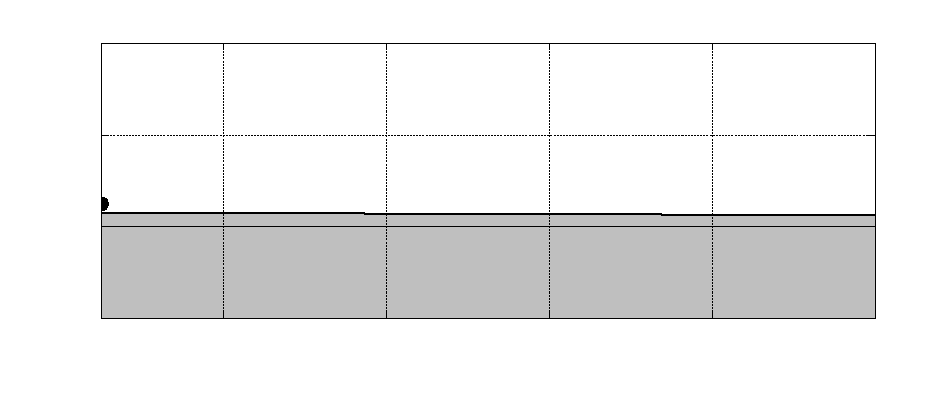
\includegraphics{./Analytic000}}%
    \gplfronttext
  \end{picture}%
\endgroup

  \caption{$t=-1$ s.}
 \end{subfigure} \\
 \begin{subfigure}{\textwidth}
  % GNUPLOT: LaTeX picture with Postscript
\begingroup
  \makeatletter
  \providecommand\color[2][]{%
    \GenericError{(gnuplot) \space\space\space\@spaces}{%
      Package color not loaded in conjunction with
      terminal option `colourtext'%
    }{See the gnuplot documentation for explanation.%
    }{Either use 'blacktext' in gnuplot or load the package
      color.sty in LaTeX.}%
    \renewcommand\color[2][]{}%
  }%
  \providecommand\includegraphics[2][]{%
    \GenericError{(gnuplot) \space\space\space\@spaces}{%
      Package graphicx or graphics not loaded%
    }{See the gnuplot documentation for explanation.%
    }{The gnuplot epslatex terminal needs graphicx.sty or graphics.sty.}%
    \renewcommand\includegraphics[2][]{}%
  }%
  \providecommand\rotatebox[2]{#2}%
  \@ifundefined{ifGPcolor}{%
    \newif\ifGPcolor
    \GPcolortrue
  }{}%
  \@ifundefined{ifGPblacktext}{%
    \newif\ifGPblacktext
    \GPblacktexttrue
  }{}%
  % define a \g@addto@macro without @ in the name:
  \let\gplgaddtomacro\g@addto@macro
  % define empty templates for all commands taking text:
  \gdef\gplbacktext{}%
  \gdef\gplfronttext{}%
  \makeatother
  \ifGPblacktext
    % no textcolor at all
    \def\colorrgb#1{}%
    \def\colorgray#1{}%
  \else
    % gray or color?
    \ifGPcolor
      \def\colorrgb#1{\color[rgb]{#1}}%
      \def\colorgray#1{\color[gray]{#1}}%
      \expandafter\def\csname LTw\endcsname{\color{white}}%
      \expandafter\def\csname LTb\endcsname{\color{black}}%
      \expandafter\def\csname LTa\endcsname{\color{black}}%
      \expandafter\def\csname LT0\endcsname{\color[rgb]{1,0,0}}%
      \expandafter\def\csname LT1\endcsname{\color[rgb]{0,1,0}}%
      \expandafter\def\csname LT2\endcsname{\color[rgb]{0,0,1}}%
      \expandafter\def\csname LT3\endcsname{\color[rgb]{1,0,1}}%
      \expandafter\def\csname LT4\endcsname{\color[rgb]{0,1,1}}%
      \expandafter\def\csname LT5\endcsname{\color[rgb]{1,1,0}}%
      \expandafter\def\csname LT6\endcsname{\color[rgb]{0,0,0}}%
      \expandafter\def\csname LT7\endcsname{\color[rgb]{1,0.3,0}}%
      \expandafter\def\csname LT8\endcsname{\color[rgb]{0.5,0.5,0.5}}%
    \else
      % gray
      \def\colorrgb#1{\color{black}}%
      \def\colorgray#1{\color[gray]{#1}}%
      \expandafter\def\csname LTw\endcsname{\color{white}}%
      \expandafter\def\csname LTb\endcsname{\color{black}}%
      \expandafter\def\csname LTa\endcsname{\color{black}}%
      \expandafter\def\csname LT0\endcsname{\color{black}}%
      \expandafter\def\csname LT1\endcsname{\color{black}}%
      \expandafter\def\csname LT2\endcsname{\color{black}}%
      \expandafter\def\csname LT3\endcsname{\color{black}}%
      \expandafter\def\csname LT4\endcsname{\color{black}}%
      \expandafter\def\csname LT5\endcsname{\color{black}}%
      \expandafter\def\csname LT6\endcsname{\color{black}}%
      \expandafter\def\csname LT7\endcsname{\color{black}}%
      \expandafter\def\csname LT8\endcsname{\color{black}}%
    \fi
  \fi
    \setlength{\unitlength}{0.0500bp}%
    \ifx\gptboxheight\undefined%
      \newlength{\gptboxheight}%
      \newlength{\gptboxwidth}%
      \newsavebox{\gptboxtext}%
    \fi%
    \setlength{\fboxrule}{0.5pt}%
    \setlength{\fboxsep}{1pt}%
\begin{picture}(8640.00,3600.00)%
    \gplgaddtomacro\gplbacktext{%
    }%
    \gplgaddtomacro\gplfronttext{%
      \csname LTb\endcsname%
      \put(176,2019){\makebox(0,0){\strut{}$\eta \cdot \frac{v^2}{Gm}$}}%
      \put(4528,154){\makebox(0,0){\strut{}$r \cdot \frac{g}{v^2}$}}%
      \csname LTb\endcsname%
      \put(682,704){\makebox(0,0)[r]{\strut{}$-4$}}%
      \csname LTb\endcsname%
      \put(682,1581){\makebox(0,0)[r]{\strut{}$0$}}%
      \csname LTb\endcsname%
      \put(682,2458){\makebox(0,0)[r]{\strut{}$4$}}%
      \csname LTb\endcsname%
      \put(682,3335){\makebox(0,0)[r]{\strut{}$8$}}%
      \csname LTb\endcsname%
      \put(1987,484){\makebox(0,0){\strut{}$0.2$}}%
      \csname LTb\endcsname%
      \put(3551,484){\makebox(0,0){\strut{}$0.4$}}%
      \csname LTb\endcsname%
      \put(5115,484){\makebox(0,0){\strut{}$0.6$}}%
      \csname LTb\endcsname%
      \put(6679,484){\makebox(0,0){\strut{}$0.8$}}%
      \csname LTb\endcsname%
      \put(8243,484){\makebox(0,0){\strut{}$1$}}%
    }%
    \gplbacktext
    \put(0,0){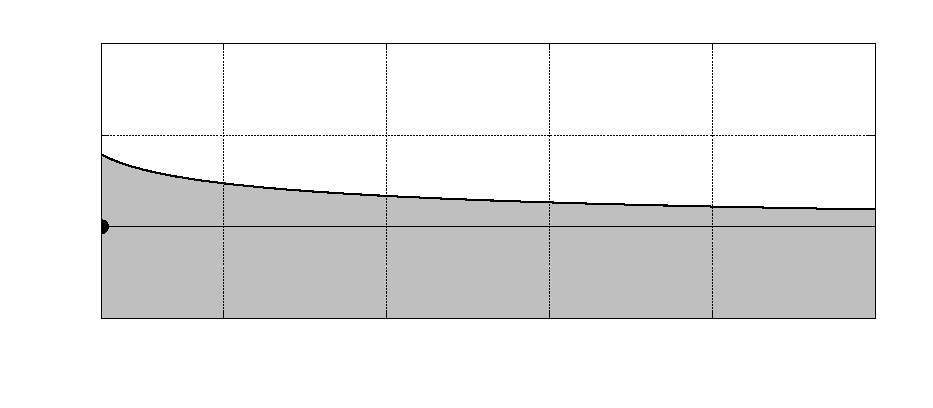
\includegraphics{./Analytic001}}%
    \gplfronttext
  \end{picture}%
\endgroup

  \caption{$t=0$ s.}
 \end{subfigure} \\
 \begin{subfigure}{\textwidth}
  % GNUPLOT: LaTeX picture with Postscript
\begingroup
  \makeatletter
  \providecommand\color[2][]{%
    \GenericError{(gnuplot) \space\space\space\@spaces}{%
      Package color not loaded in conjunction with
      terminal option `colourtext'%
    }{See the gnuplot documentation for explanation.%
    }{Either use 'blacktext' in gnuplot or load the package
      color.sty in LaTeX.}%
    \renewcommand\color[2][]{}%
  }%
  \providecommand\includegraphics[2][]{%
    \GenericError{(gnuplot) \space\space\space\@spaces}{%
      Package graphicx or graphics not loaded%
    }{See the gnuplot documentation for explanation.%
    }{The gnuplot epslatex terminal needs graphicx.sty or graphics.sty.}%
    \renewcommand\includegraphics[2][]{}%
  }%
  \providecommand\rotatebox[2]{#2}%
  \@ifundefined{ifGPcolor}{%
    \newif\ifGPcolor
    \GPcolortrue
  }{}%
  \@ifundefined{ifGPblacktext}{%
    \newif\ifGPblacktext
    \GPblacktexttrue
  }{}%
  % define a \g@addto@macro without @ in the name:
  \let\gplgaddtomacro\g@addto@macro
  % define empty templates for all commands taking text:
  \gdef\gplbacktext{}%
  \gdef\gplfronttext{}%
  \makeatother
  \ifGPblacktext
    % no textcolor at all
    \def\colorrgb#1{}%
    \def\colorgray#1{}%
  \else
    % gray or color?
    \ifGPcolor
      \def\colorrgb#1{\color[rgb]{#1}}%
      \def\colorgray#1{\color[gray]{#1}}%
      \expandafter\def\csname LTw\endcsname{\color{white}}%
      \expandafter\def\csname LTb\endcsname{\color{black}}%
      \expandafter\def\csname LTa\endcsname{\color{black}}%
      \expandafter\def\csname LT0\endcsname{\color[rgb]{1,0,0}}%
      \expandafter\def\csname LT1\endcsname{\color[rgb]{0,1,0}}%
      \expandafter\def\csname LT2\endcsname{\color[rgb]{0,0,1}}%
      \expandafter\def\csname LT3\endcsname{\color[rgb]{1,0,1}}%
      \expandafter\def\csname LT4\endcsname{\color[rgb]{0,1,1}}%
      \expandafter\def\csname LT5\endcsname{\color[rgb]{1,1,0}}%
      \expandafter\def\csname LT6\endcsname{\color[rgb]{0,0,0}}%
      \expandafter\def\csname LT7\endcsname{\color[rgb]{1,0.3,0}}%
      \expandafter\def\csname LT8\endcsname{\color[rgb]{0.5,0.5,0.5}}%
    \else
      % gray
      \def\colorrgb#1{\color{black}}%
      \def\colorgray#1{\color[gray]{#1}}%
      \expandafter\def\csname LTw\endcsname{\color{white}}%
      \expandafter\def\csname LTb\endcsname{\color{black}}%
      \expandafter\def\csname LTa\endcsname{\color{black}}%
      \expandafter\def\csname LT0\endcsname{\color{black}}%
      \expandafter\def\csname LT1\endcsname{\color{black}}%
      \expandafter\def\csname LT2\endcsname{\color{black}}%
      \expandafter\def\csname LT3\endcsname{\color{black}}%
      \expandafter\def\csname LT4\endcsname{\color{black}}%
      \expandafter\def\csname LT5\endcsname{\color{black}}%
      \expandafter\def\csname LT6\endcsname{\color{black}}%
      \expandafter\def\csname LT7\endcsname{\color{black}}%
      \expandafter\def\csname LT8\endcsname{\color{black}}%
    \fi
  \fi
    \setlength{\unitlength}{0.0500bp}%
    \ifx\gptboxheight\undefined%
      \newlength{\gptboxheight}%
      \newlength{\gptboxwidth}%
      \newsavebox{\gptboxtext}%
    \fi%
    \setlength{\fboxrule}{0.5pt}%
    \setlength{\fboxsep}{1pt}%
\begin{picture}(8640.00,3600.00)%
    \gplgaddtomacro\gplbacktext{%
    }%
    \gplgaddtomacro\gplfronttext{%
      \csname LTb\endcsname%
      \put(176,2019){\makebox(0,0){\strut{}$\eta \cdot \frac{v^2}{Gm}$}}%
      \put(4528,154){\makebox(0,0){\strut{}$r \cdot \frac{g}{v^2}$}}%
      \csname LTb\endcsname%
      \put(682,704){\makebox(0,0)[r]{\strut{}$-4$}}%
      \csname LTb\endcsname%
      \put(682,1581){\makebox(0,0)[r]{\strut{}$0$}}%
      \csname LTb\endcsname%
      \put(682,2458){\makebox(0,0)[r]{\strut{}$4$}}%
      \csname LTb\endcsname%
      \put(682,3335){\makebox(0,0)[r]{\strut{}$8$}}%
      \csname LTb\endcsname%
      \put(1987,484){\makebox(0,0){\strut{}$0.2$}}%
      \csname LTb\endcsname%
      \put(3551,484){\makebox(0,0){\strut{}$0.4$}}%
      \csname LTb\endcsname%
      \put(5115,484){\makebox(0,0){\strut{}$0.6$}}%
      \csname LTb\endcsname%
      \put(6679,484){\makebox(0,0){\strut{}$0.8$}}%
      \csname LTb\endcsname%
      \put(8243,484){\makebox(0,0){\strut{}$1$}}%
    }%
    \gplbacktext
    \put(0,0){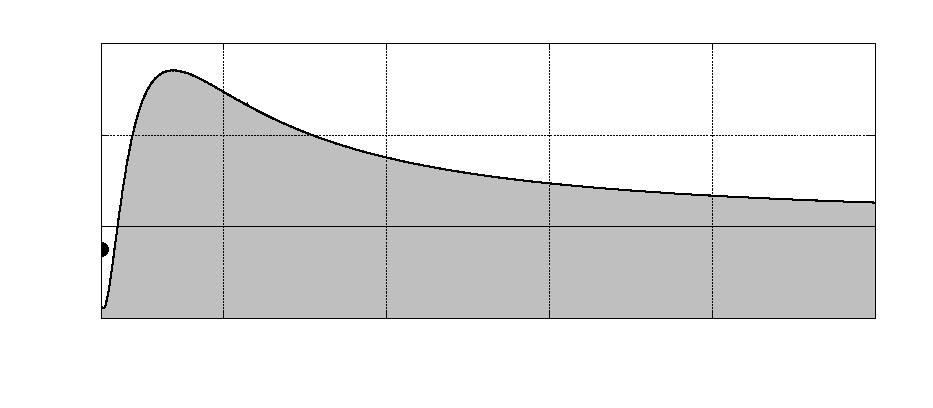
\includegraphics{./Analytic002}}%
    \gplfronttext
  \end{picture}%
\endgroup

  \caption{$t=1$ s.}
 \end{subfigure}
\end{centering}
\end{figure}

\begin{figure}[p] \ContinuedFloat
\begin{centering}
 \begin{subfigure}{\textwidth}
  % GNUPLOT: LaTeX picture with Postscript
\begingroup
  \makeatletter
  \providecommand\color[2][]{%
    \GenericError{(gnuplot) \space\space\space\@spaces}{%
      Package color not loaded in conjunction with
      terminal option `colourtext'%
    }{See the gnuplot documentation for explanation.%
    }{Either use 'blacktext' in gnuplot or load the package
      color.sty in LaTeX.}%
    \renewcommand\color[2][]{}%
  }%
  \providecommand\includegraphics[2][]{%
    \GenericError{(gnuplot) \space\space\space\@spaces}{%
      Package graphicx or graphics not loaded%
    }{See the gnuplot documentation for explanation.%
    }{The gnuplot epslatex terminal needs graphicx.sty or graphics.sty.}%
    \renewcommand\includegraphics[2][]{}%
  }%
  \providecommand\rotatebox[2]{#2}%
  \@ifundefined{ifGPcolor}{%
    \newif\ifGPcolor
    \GPcolortrue
  }{}%
  \@ifundefined{ifGPblacktext}{%
    \newif\ifGPblacktext
    \GPblacktexttrue
  }{}%
  % define a \g@addto@macro without @ in the name:
  \let\gplgaddtomacro\g@addto@macro
  % define empty templates for all commands taking text:
  \gdef\gplbacktext{}%
  \gdef\gplfronttext{}%
  \makeatother
  \ifGPblacktext
    % no textcolor at all
    \def\colorrgb#1{}%
    \def\colorgray#1{}%
  \else
    % gray or color?
    \ifGPcolor
      \def\colorrgb#1{\color[rgb]{#1}}%
      \def\colorgray#1{\color[gray]{#1}}%
      \expandafter\def\csname LTw\endcsname{\color{white}}%
      \expandafter\def\csname LTb\endcsname{\color{black}}%
      \expandafter\def\csname LTa\endcsname{\color{black}}%
      \expandafter\def\csname LT0\endcsname{\color[rgb]{1,0,0}}%
      \expandafter\def\csname LT1\endcsname{\color[rgb]{0,1,0}}%
      \expandafter\def\csname LT2\endcsname{\color[rgb]{0,0,1}}%
      \expandafter\def\csname LT3\endcsname{\color[rgb]{1,0,1}}%
      \expandafter\def\csname LT4\endcsname{\color[rgb]{0,1,1}}%
      \expandafter\def\csname LT5\endcsname{\color[rgb]{1,1,0}}%
      \expandafter\def\csname LT6\endcsname{\color[rgb]{0,0,0}}%
      \expandafter\def\csname LT7\endcsname{\color[rgb]{1,0.3,0}}%
      \expandafter\def\csname LT8\endcsname{\color[rgb]{0.5,0.5,0.5}}%
    \else
      % gray
      \def\colorrgb#1{\color{black}}%
      \def\colorgray#1{\color[gray]{#1}}%
      \expandafter\def\csname LTw\endcsname{\color{white}}%
      \expandafter\def\csname LTb\endcsname{\color{black}}%
      \expandafter\def\csname LTa\endcsname{\color{black}}%
      \expandafter\def\csname LT0\endcsname{\color{black}}%
      \expandafter\def\csname LT1\endcsname{\color{black}}%
      \expandafter\def\csname LT2\endcsname{\color{black}}%
      \expandafter\def\csname LT3\endcsname{\color{black}}%
      \expandafter\def\csname LT4\endcsname{\color{black}}%
      \expandafter\def\csname LT5\endcsname{\color{black}}%
      \expandafter\def\csname LT6\endcsname{\color{black}}%
      \expandafter\def\csname LT7\endcsname{\color{black}}%
      \expandafter\def\csname LT8\endcsname{\color{black}}%
    \fi
  \fi
    \setlength{\unitlength}{0.0500bp}%
    \ifx\gptboxheight\undefined%
      \newlength{\gptboxheight}%
      \newlength{\gptboxwidth}%
      \newsavebox{\gptboxtext}%
    \fi%
    \setlength{\fboxrule}{0.5pt}%
    \setlength{\fboxsep}{1pt}%
\begin{picture}(8640.00,3600.00)%
    \gplgaddtomacro\gplbacktext{%
    }%
    \gplgaddtomacro\gplfronttext{%
      \csname LTb\endcsname%
      \put(176,2019){\makebox(0,0){\strut{}$\frac{\eta}{Gm/v^2}$}}%
      \put(4528,154){\makebox(0,0){\strut{}$\chi$}}%
      \csname LTb\endcsname%
      \put(682,704){\makebox(0,0)[r]{\strut{}$-4$}}%
      \csname LTb\endcsname%
      \put(682,1581){\makebox(0,0)[r]{\strut{}$0$}}%
      \csname LTb\endcsname%
      \put(682,2458){\makebox(0,0)[r]{\strut{}$4$}}%
      \csname LTb\endcsname%
      \put(682,3335){\makebox(0,0)[r]{\strut{}$8$}}%
      \csname LTb\endcsname%
      \put(1987,484){\makebox(0,0){\strut{}$0.2$}}%
      \csname LTb\endcsname%
      \put(3551,484){\makebox(0,0){\strut{}$0.4$}}%
      \csname LTb\endcsname%
      \put(5115,484){\makebox(0,0){\strut{}$0.6$}}%
      \csname LTb\endcsname%
      \put(6679,484){\makebox(0,0){\strut{}$0.8$}}%
      \csname LTb\endcsname%
      \put(8243,484){\makebox(0,0){\strut{}$1$}}%
    }%
    \gplbacktext
    \put(0,0){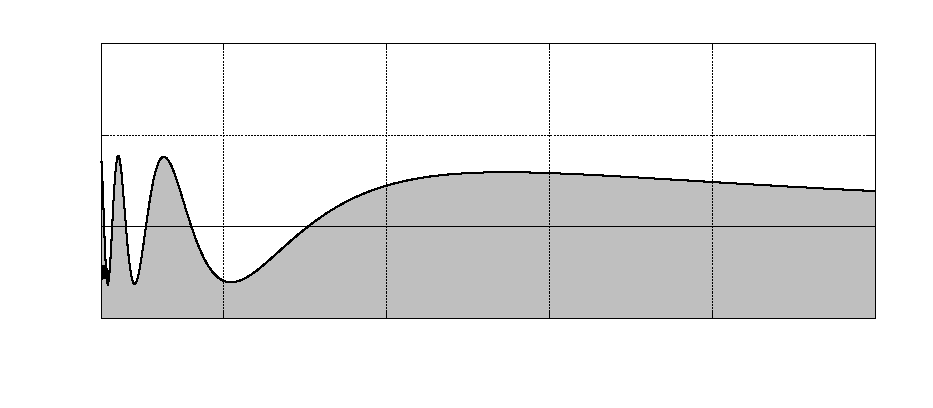
\includegraphics{./3Analytic/Analytic003}}%
    \gplfronttext
  \end{picture}%
\endgroup

  \caption{$t=2$ s.}
 \end{subfigure} \\
 \begin{subfigure}{\textwidth}
  % GNUPLOT: LaTeX picture with Postscript
\begingroup
  \makeatletter
  \providecommand\color[2][]{%
    \GenericError{(gnuplot) \space\space\space\@spaces}{%
      Package color not loaded in conjunction with
      terminal option `colourtext'%
    }{See the gnuplot documentation for explanation.%
    }{Either use 'blacktext' in gnuplot or load the package
      color.sty in LaTeX.}%
    \renewcommand\color[2][]{}%
  }%
  \providecommand\includegraphics[2][]{%
    \GenericError{(gnuplot) \space\space\space\@spaces}{%
      Package graphicx or graphics not loaded%
    }{See the gnuplot documentation for explanation.%
    }{The gnuplot epslatex terminal needs graphicx.sty or graphics.sty.}%
    \renewcommand\includegraphics[2][]{}%
  }%
  \providecommand\rotatebox[2]{#2}%
  \@ifundefined{ifGPcolor}{%
    \newif\ifGPcolor
    \GPcolortrue
  }{}%
  \@ifundefined{ifGPblacktext}{%
    \newif\ifGPblacktext
    \GPblacktexttrue
  }{}%
  % define a \g@addto@macro without @ in the name:
  \let\gplgaddtomacro\g@addto@macro
  % define empty templates for all commands taking text:
  \gdef\gplbacktext{}%
  \gdef\gplfronttext{}%
  \makeatother
  \ifGPblacktext
    % no textcolor at all
    \def\colorrgb#1{}%
    \def\colorgray#1{}%
  \else
    % gray or color?
    \ifGPcolor
      \def\colorrgb#1{\color[rgb]{#1}}%
      \def\colorgray#1{\color[gray]{#1}}%
      \expandafter\def\csname LTw\endcsname{\color{white}}%
      \expandafter\def\csname LTb\endcsname{\color{black}}%
      \expandafter\def\csname LTa\endcsname{\color{black}}%
      \expandafter\def\csname LT0\endcsname{\color[rgb]{1,0,0}}%
      \expandafter\def\csname LT1\endcsname{\color[rgb]{0,1,0}}%
      \expandafter\def\csname LT2\endcsname{\color[rgb]{0,0,1}}%
      \expandafter\def\csname LT3\endcsname{\color[rgb]{1,0,1}}%
      \expandafter\def\csname LT4\endcsname{\color[rgb]{0,1,1}}%
      \expandafter\def\csname LT5\endcsname{\color[rgb]{1,1,0}}%
      \expandafter\def\csname LT6\endcsname{\color[rgb]{0,0,0}}%
      \expandafter\def\csname LT7\endcsname{\color[rgb]{1,0.3,0}}%
      \expandafter\def\csname LT8\endcsname{\color[rgb]{0.5,0.5,0.5}}%
    \else
      % gray
      \def\colorrgb#1{\color{black}}%
      \def\colorgray#1{\color[gray]{#1}}%
      \expandafter\def\csname LTw\endcsname{\color{white}}%
      \expandafter\def\csname LTb\endcsname{\color{black}}%
      \expandafter\def\csname LTa\endcsname{\color{black}}%
      \expandafter\def\csname LT0\endcsname{\color{black}}%
      \expandafter\def\csname LT1\endcsname{\color{black}}%
      \expandafter\def\csname LT2\endcsname{\color{black}}%
      \expandafter\def\csname LT3\endcsname{\color{black}}%
      \expandafter\def\csname LT4\endcsname{\color{black}}%
      \expandafter\def\csname LT5\endcsname{\color{black}}%
      \expandafter\def\csname LT6\endcsname{\color{black}}%
      \expandafter\def\csname LT7\endcsname{\color{black}}%
      \expandafter\def\csname LT8\endcsname{\color{black}}%
    \fi
  \fi
    \setlength{\unitlength}{0.0500bp}%
    \ifx\gptboxheight\undefined%
      \newlength{\gptboxheight}%
      \newlength{\gptboxwidth}%
      \newsavebox{\gptboxtext}%
    \fi%
    \setlength{\fboxrule}{0.5pt}%
    \setlength{\fboxsep}{1pt}%
\begin{picture}(8640.00,3600.00)%
    \gplgaddtomacro\gplbacktext{%
    }%
    \gplgaddtomacro\gplfronttext{%
      \csname LTb\endcsname%
      \put(176,2019){\makebox(0,0){\strut{}$\eta \cdot \frac{v^2}{Gm}$}}%
      \put(4528,154){\makebox(0,0){\strut{}$r \cdot \frac{g}{v^2}$}}%
      \csname LTb\endcsname%
      \put(682,704){\makebox(0,0)[r]{\strut{}$-4$}}%
      \csname LTb\endcsname%
      \put(682,1581){\makebox(0,0)[r]{\strut{}$0$}}%
      \csname LTb\endcsname%
      \put(682,2458){\makebox(0,0)[r]{\strut{}$4$}}%
      \csname LTb\endcsname%
      \put(682,3335){\makebox(0,0)[r]{\strut{}$8$}}%
      \csname LTb\endcsname%
      \put(1987,484){\makebox(0,0){\strut{}$0.2$}}%
      \csname LTb\endcsname%
      \put(3551,484){\makebox(0,0){\strut{}$0.4$}}%
      \csname LTb\endcsname%
      \put(5115,484){\makebox(0,0){\strut{}$0.6$}}%
      \csname LTb\endcsname%
      \put(6679,484){\makebox(0,0){\strut{}$0.8$}}%
      \csname LTb\endcsname%
      \put(8243,484){\makebox(0,0){\strut{}$1$}}%
    }%
    \gplbacktext
    \put(0,0){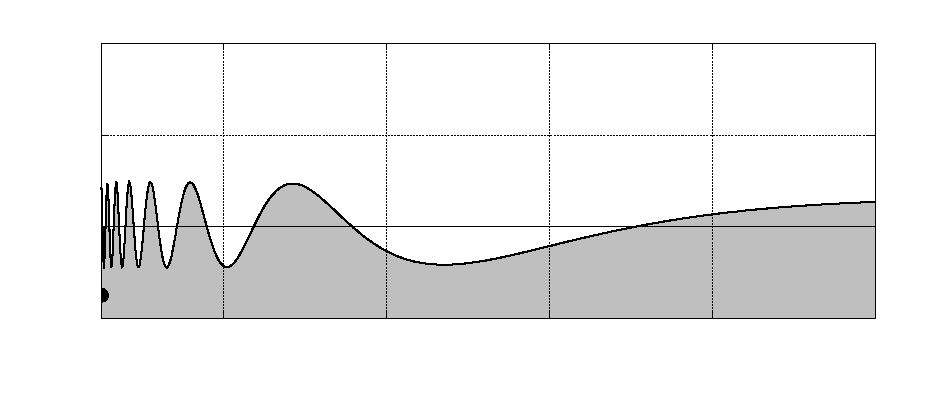
\includegraphics{./Analytic004}}%
    \gplfronttext
  \end{picture}%
\endgroup

  \caption{$t=3$ s.}
 \end{subfigure} \\
  \begin{subfigure}{\textwidth}
  % GNUPLOT: LaTeX picture with Postscript
\begingroup
  \makeatletter
  \providecommand\color[2][]{%
    \GenericError{(gnuplot) \space\space\space\@spaces}{%
      Package color not loaded in conjunction with
      terminal option `colourtext'%
    }{See the gnuplot documentation for explanation.%
    }{Either use 'blacktext' in gnuplot or load the package
      color.sty in LaTeX.}%
    \renewcommand\color[2][]{}%
  }%
  \providecommand\includegraphics[2][]{%
    \GenericError{(gnuplot) \space\space\space\@spaces}{%
      Package graphicx or graphics not loaded%
    }{See the gnuplot documentation for explanation.%
    }{The gnuplot epslatex terminal needs graphicx.sty or graphics.sty.}%
    \renewcommand\includegraphics[2][]{}%
  }%
  \providecommand\rotatebox[2]{#2}%
  \@ifundefined{ifGPcolor}{%
    \newif\ifGPcolor
    \GPcolortrue
  }{}%
  \@ifundefined{ifGPblacktext}{%
    \newif\ifGPblacktext
    \GPblacktexttrue
  }{}%
  % define a \g@addto@macro without @ in the name:
  \let\gplgaddtomacro\g@addto@macro
  % define empty templates for all commands taking text:
  \gdef\gplbacktext{}%
  \gdef\gplfronttext{}%
  \makeatother
  \ifGPblacktext
    % no textcolor at all
    \def\colorrgb#1{}%
    \def\colorgray#1{}%
  \else
    % gray or color?
    \ifGPcolor
      \def\colorrgb#1{\color[rgb]{#1}}%
      \def\colorgray#1{\color[gray]{#1}}%
      \expandafter\def\csname LTw\endcsname{\color{white}}%
      \expandafter\def\csname LTb\endcsname{\color{black}}%
      \expandafter\def\csname LTa\endcsname{\color{black}}%
      \expandafter\def\csname LT0\endcsname{\color[rgb]{1,0,0}}%
      \expandafter\def\csname LT1\endcsname{\color[rgb]{0,1,0}}%
      \expandafter\def\csname LT2\endcsname{\color[rgb]{0,0,1}}%
      \expandafter\def\csname LT3\endcsname{\color[rgb]{1,0,1}}%
      \expandafter\def\csname LT4\endcsname{\color[rgb]{0,1,1}}%
      \expandafter\def\csname LT5\endcsname{\color[rgb]{1,1,0}}%
      \expandafter\def\csname LT6\endcsname{\color[rgb]{0,0,0}}%
      \expandafter\def\csname LT7\endcsname{\color[rgb]{1,0.3,0}}%
      \expandafter\def\csname LT8\endcsname{\color[rgb]{0.5,0.5,0.5}}%
    \else
      % gray
      \def\colorrgb#1{\color{black}}%
      \def\colorgray#1{\color[gray]{#1}}%
      \expandafter\def\csname LTw\endcsname{\color{white}}%
      \expandafter\def\csname LTb\endcsname{\color{black}}%
      \expandafter\def\csname LTa\endcsname{\color{black}}%
      \expandafter\def\csname LT0\endcsname{\color{black}}%
      \expandafter\def\csname LT1\endcsname{\color{black}}%
      \expandafter\def\csname LT2\endcsname{\color{black}}%
      \expandafter\def\csname LT3\endcsname{\color{black}}%
      \expandafter\def\csname LT4\endcsname{\color{black}}%
      \expandafter\def\csname LT5\endcsname{\color{black}}%
      \expandafter\def\csname LT6\endcsname{\color{black}}%
      \expandafter\def\csname LT7\endcsname{\color{black}}%
      \expandafter\def\csname LT8\endcsname{\color{black}}%
    \fi
  \fi
    \setlength{\unitlength}{0.0500bp}%
    \ifx\gptboxheight\undefined%
      \newlength{\gptboxheight}%
      \newlength{\gptboxwidth}%
      \newsavebox{\gptboxtext}%
    \fi%
    \setlength{\fboxrule}{0.5pt}%
    \setlength{\fboxsep}{1pt}%
\begin{picture}(8640.00,3600.00)%
    \gplgaddtomacro\gplbacktext{%
    }%
    \gplgaddtomacro\gplfronttext{%
      \csname LTb\endcsname%
      \put(176,2019){\makebox(0,0){\strut{}$\eta$}}%
      \put(4528,154){\makebox(0,0){\strut{}$r$}}%
      \csname LTb\endcsname%
      \put(682,704){\makebox(0,0)[r]{\strut{}$-4$}}%
      \csname LTb\endcsname%
      \put(682,1581){\makebox(0,0)[r]{\strut{}$0$}}%
      \csname LTb\endcsname%
      \put(682,2458){\makebox(0,0)[r]{\strut{}$4$}}%
      \csname LTb\endcsname%
      \put(682,3335){\makebox(0,0)[r]{\strut{}$8$}}%
      \csname LTb\endcsname%
      \put(1987,484){\makebox(0,0){\strut{}$0.2$}}%
      \csname LTb\endcsname%
      \put(3551,484){\makebox(0,0){\strut{}$0.4$}}%
      \csname LTb\endcsname%
      \put(5115,484){\makebox(0,0){\strut{}$0.6$}}%
      \csname LTb\endcsname%
      \put(6679,484){\makebox(0,0){\strut{}$0.8$}}%
      \csname LTb\endcsname%
      \put(8243,484){\makebox(0,0){\strut{}$1$}}%
    }%
    \gplbacktext
    \put(0,0){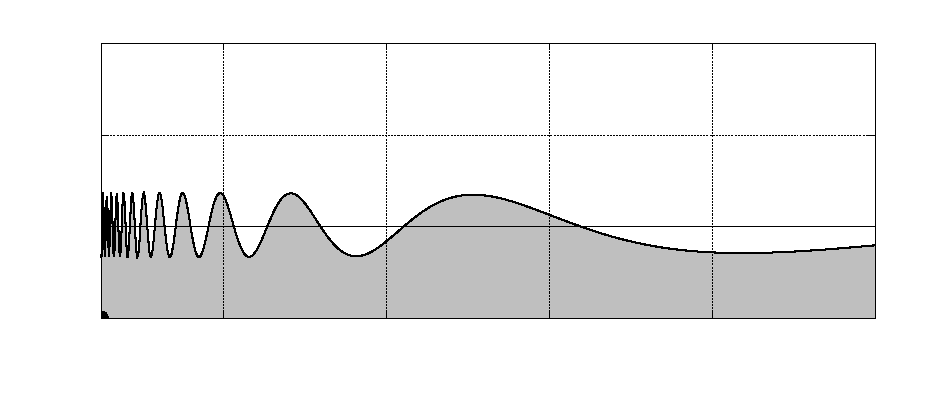
\includegraphics{./Analytic005}}%
    \gplfronttext
  \end{picture}%
\endgroup

  \caption{$t=4$ s.}
 \end{subfigure}
 \end{centering}
 \caption{Deformation of the neutron star around the time of impact.}
 \label{fig:eta}
\end{figure}

\subsection{Calculating the Energy Transferred}
\label{chap:energy}

Finally, the last quantity of interest is the energy. Having an idea of what the waves would look like is great, however, if such a collision were to take place, the waves would not be detectable from Earth. On the other hand, the energy would. Now, clearly in order to make reasonable predictions about what would be detected on Earth, more than just Newtonian gravity is necessary. Since energy does not escape the system in this model, it is only transferred between the primordial black hole and the neutron star, we cannot predict what such an event would look like from Earth, but it is a worthwhile calculation nonetheless. \\

To calculate the energy transferred we shall start with
\begin{align*}
E(t) &= \frac{1}{2} \rho \int_V \left| \grad \varphi \right|^2 + \rho g \int_V z,
\end{align*}
where $\grad \varphi$ is of course $\overset{\rightharpoonup}u$, which is the typical expression for energy, except we use the density of a fluid element instead of its mass. We can expand the volume integral out so that 
\begin{align*}
E(t) &= \frac{1}{2} \rho \int_0^{2\pi} \int_0^\infty \int_{-\infty}^0 \left| \grad \varphi \right|^2 \, dz \, r \, dr \, d\theta + \rho g \int_0^{2\pi} \int_0^\infty \int_0^\eta z \, dz \, r \, dr \, d\theta,
\end{align*}
notice that the bounds on $z$ are from $0$ to $\eta$, this is because we are interested in the change in energy so we subtract the initial potential energy of the neutron star. After solving the trivia integrals we find that
\begin{align*}
E(t) &= \rho \pi \left( \int_0^\infty \int_{-\infty}^0 \left( \frac{\partial \varphi}{\partial r} \right)^2 r \, dz \, dr + \int_0^\infty \int_{-\infty}^0 \left( \frac{\partial \varphi}{\partial z} \right)^2 r \, dz \, dr + g \int_0^\infty \eta^2 r \, dr \right).
\end{align*}
These are non-trivial integrals since $\varphi$, and $\eta$ are themselves non-trivial integrals. To simplify and tidy this calculation, let $\clubsuit$, $\spadesuit$, and $\blacklozenge$ be the three terms respectively, so that $E = \rho \pi (\clubsuit + \spadesuit + g \blacklozenge)$. \\

The reason we wrote the velocity potential, and the deformation of the surface as Hankel transforms of their time components is so these integrals can more easily be solved using Theorem ***. Starting with the first term,
\begin{align*}
\clubsuit &= \int_0^\infty \int_{-\infty}^0 \left( \frac{\partial \varphi}{\partial r} \right)^2 r \, dz \, dr,
\end{align*}
$\partial \varphi / \partial r$ can be replaced by its Hankel transform representation so that
\begin{align*}
\clubsuit &= \int_{-\infty}^0 \int_0^\infty \Hank[1]{e^{kz}T(t;k)}^2(r,z,t) r \, dr \, dz.
\end{align*}
After invoking Theorem *** we acquire
\begin{align*}
\clubsuit &= \int_{-\infty}^0 \int_0^\infty e^{2kz} T^2(t;k) \, k \, dk \, dz,
\end{align*}
then by integrating over $z$ we get the final expression
\begin{align*}
\clubsuit &= \frac{1}{2} \int_0^\infty T^2(t;k) \, dk.
\end{align*}

Following this same procedure for the other two terms we find that 
\begin{align*}
\spadesuit &= \frac{1}{2} \int_0^\infty T^2(t;k) \, dk, \text{ and} \\
\blacklozenge &= \int_0^\infty \frac{\widetilde{T}^2(t;k)}{k} \, dk.
\end{align*}



\begin{align*}
E(t) = \rho \pi \int_0^\infty T^2(t;k) + g \frac{\widetilde{T}^2(t;k)}{k} \, dk
\end{align*}
\begin{equation}
\label{eq:fullenergy}
\begin{split}
E = \frac{G^2 m^2 \rho \pi}{g} \int_0^\infty \frac{v^2}{g} \left( \frac{- \sgn(t) e^{-kv |t|} + 2 \Heavi(t) \cos(\omega_k t)}{1+kv^2/g} \right)^2& \\
+ \frac{1}{k} \left( \frac{e^{-kv |t|} + 2 \Heavi(t) v \sqrt{\frac{k}{g}} \sin(\omega_k t)}{1+kv^2/g} \right)^2& \, dk
\end{split}
\end{equation}

By taking the long time limit the exponentials decay to zero, and the sine and cosine simplify to $1$. The energy then becomes
\begin{align}
\label{eq:energy}
E = 4 \pi \rho \frac{G^2 m^2}{g}.
\end{align}


\begin{figure}[p]
 % GNUPLOT: LaTeX picture with Postscript
\begingroup
  \makeatletter
  \providecommand\color[2][]{%
    \GenericError{(gnuplot) \space\space\space\@spaces}{%
      Package color not loaded in conjunction with
      terminal option `colourtext'%
    }{See the gnuplot documentation for explanation.%
    }{Either use 'blacktext' in gnuplot or load the package
      color.sty in LaTeX.}%
    \renewcommand\color[2][]{}%
  }%
  \providecommand\includegraphics[2][]{%
    \GenericError{(gnuplot) \space\space\space\@spaces}{%
      Package graphicx or graphics not loaded%
    }{See the gnuplot documentation for explanation.%
    }{The gnuplot epslatex terminal needs graphicx.sty or graphics.sty.}%
    \renewcommand\includegraphics[2][]{}%
  }%
  \providecommand\rotatebox[2]{#2}%
  \@ifundefined{ifGPcolor}{%
    \newif\ifGPcolor
    \GPcolortrue
  }{}%
  \@ifundefined{ifGPblacktext}{%
    \newif\ifGPblacktext
    \GPblacktexttrue
  }{}%
  % define a \g@addto@macro without @ in the name:
  \let\gplgaddtomacro\g@addto@macro
  % define empty templates for all commands taking text:
  \gdef\gplbacktext{}%
  \gdef\gplfronttext{}%
  \makeatother
  \ifGPblacktext
    % no textcolor at all
    \def\colorrgb#1{}%
    \def\colorgray#1{}%
  \else
    % gray or color?
    \ifGPcolor
      \def\colorrgb#1{\color[rgb]{#1}}%
      \def\colorgray#1{\color[gray]{#1}}%
      \expandafter\def\csname LTw\endcsname{\color{white}}%
      \expandafter\def\csname LTb\endcsname{\color{black}}%
      \expandafter\def\csname LTa\endcsname{\color{black}}%
      \expandafter\def\csname LT0\endcsname{\color[rgb]{1,0,0}}%
      \expandafter\def\csname LT1\endcsname{\color[rgb]{0,1,0}}%
      \expandafter\def\csname LT2\endcsname{\color[rgb]{0,0,1}}%
      \expandafter\def\csname LT3\endcsname{\color[rgb]{1,0,1}}%
      \expandafter\def\csname LT4\endcsname{\color[rgb]{0,1,1}}%
      \expandafter\def\csname LT5\endcsname{\color[rgb]{1,1,0}}%
      \expandafter\def\csname LT6\endcsname{\color[rgb]{0,0,0}}%
      \expandafter\def\csname LT7\endcsname{\color[rgb]{1,0.3,0}}%
      \expandafter\def\csname LT8\endcsname{\color[rgb]{0.5,0.5,0.5}}%
    \else
      % gray
      \def\colorrgb#1{\color{black}}%
      \def\colorgray#1{\color[gray]{#1}}%
      \expandafter\def\csname LTw\endcsname{\color{white}}%
      \expandafter\def\csname LTb\endcsname{\color{black}}%
      \expandafter\def\csname LTa\endcsname{\color{black}}%
      \expandafter\def\csname LT0\endcsname{\color{black}}%
      \expandafter\def\csname LT1\endcsname{\color{black}}%
      \expandafter\def\csname LT2\endcsname{\color{black}}%
      \expandafter\def\csname LT3\endcsname{\color{black}}%
      \expandafter\def\csname LT4\endcsname{\color{black}}%
      \expandafter\def\csname LT5\endcsname{\color{black}}%
      \expandafter\def\csname LT6\endcsname{\color{black}}%
      \expandafter\def\csname LT7\endcsname{\color{black}}%
      \expandafter\def\csname LT8\endcsname{\color{black}}%
    \fi
  \fi
    \setlength{\unitlength}{0.0500bp}%
    \ifx\gptboxheight\undefined%
      \newlength{\gptboxheight}%
      \newlength{\gptboxwidth}%
      \newsavebox{\gptboxtext}%
    \fi%
    \setlength{\fboxrule}{0.5pt}%
    \setlength{\fboxsep}{1pt}%
\begin{picture}(8640.00,6480.00)%
    \gplgaddtomacro\gplbacktext{%
    }%
    \gplgaddtomacro\gplfronttext{%
      \csname LTb\endcsname%
      \put(176,3459){\rotatebox{-270}{\makebox(0,0){\strut{}$E \cdot \frac{g}{G^2m^2 \rho}$}}}%
      \put(4594,154){\makebox(0,0){\strut{}$t \cdot \frac{g}{v}$}}%
      \csname LTb\endcsname%
      \put(814,1411){\makebox(0,0)[r]{\strut{}$100$}}%
      \csname LTb\endcsname%
      \put(814,2843){\makebox(0,0)[r]{\strut{}$120$}}%
      \csname LTb\endcsname%
      \put(814,4275){\makebox(0,0)[r]{\strut{}$140$}}%
      \csname LTb\endcsname%
      \put(814,5708){\makebox(0,0)[r]{\strut{}$160$}}%
      \csname LTb\endcsname%
      \put(946,484){\makebox(0,0){\strut{}$-30$}}%
      \csname LTb\endcsname%
      \put(2162,484){\makebox(0,0){\strut{}$-20$}}%
      \csname LTb\endcsname%
      \put(3378,484){\makebox(0,0){\strut{}$-10$}}%
      \csname LTb\endcsname%
      \put(4595,484){\makebox(0,0){\strut{}$0$}}%
      \csname LTb\endcsname%
      \put(5811,484){\makebox(0,0){\strut{}$10$}}%
      \csname LTb\endcsname%
      \put(7027,484){\makebox(0,0){\strut{}$20$}}%
      \csname LTb\endcsname%
      \put(8243,484){\makebox(0,0){\strut{}$30$}}%
    }%
    \gplbacktext
    \put(0,0){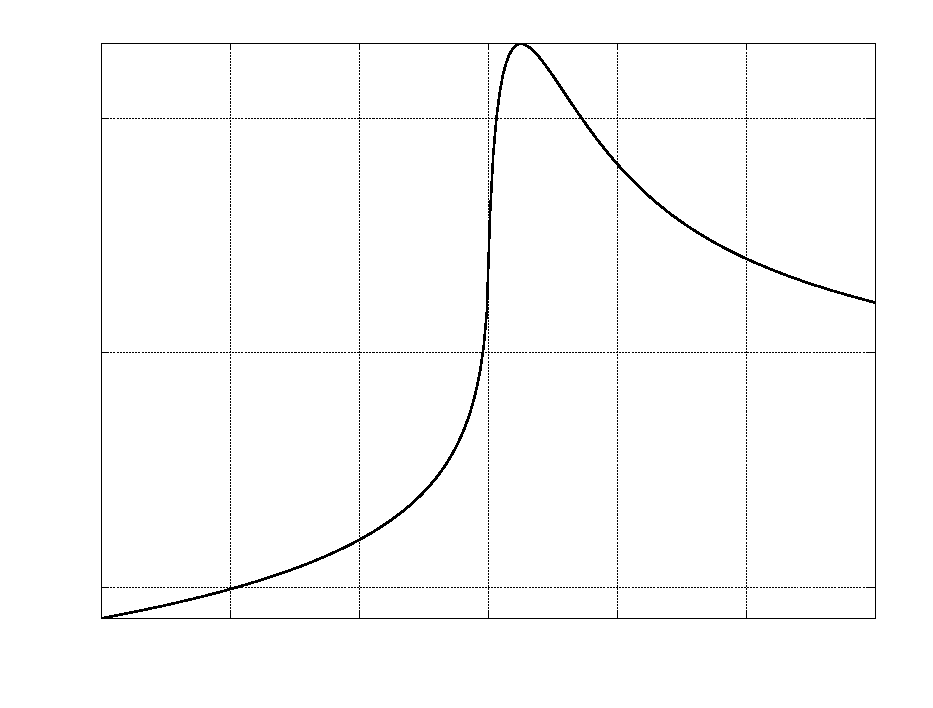
\includegraphics{./AnalyticEnergyPlot}}%
    \gplfronttext
  \end{picture}%
\endgroup

 \caption{Energy! All variables set to 1.}
 \label{fig:analyticenergy}
\end{figure}

***
Compare with dynamical friction solution




\end{document}
















